%%%%%%%%%%%%%%%%%%%%%%%%%%%%%%%%%%%%%%%%%%%%%%%%%%%%%%%%%%%%%%%%%%%%
%%
%%  Copyright (C) 2011, 2014 International Business Machines
%%
%%  Author:  Frank Liu, IBM
%%
%%  All Rights Reserved. This program and the accompanying materials
%%  are made available under the terms of the Eclipse Public License v1.0
%%  which accompanies this distribution, and is available at
%%  http://www.eclipse.org/legal/epl-v10.html
%%
%%%%%%%%%%%%%%%%%%%%%%%%%%%%%%%%%%%%%%%%%%%%%%%%%%%%%%%%%%%%%%%%%%%%

%% 
%%  User manual for SPRNT, always under revision
%% 
%% better to compile with pdflatex, latex complains.
%%
%%  pdflatex sprnt_manual.tex
%%  pdflatex sprnt_manual.tex
%%

\documentclass[10pt, letterpaper]{article}

\usepackage{graphicx}
\usepackage{amsmath}
\usepackage{color}
\usepackage{listings}
\usepackage{url}
\usepackage[letterpaper]{geometry}

\setlength{\topmargin}{-0.5in}
\setlength{\oddsidemargin}{-0.25in}
\setlength{\evensidemargin}{-0.25in}
\setlength{\textheight}{9.0in}
\setlength{\textwidth}{6.5in}

\def\epswidth{3.0in}

%% declaration of the images

\title{SPRNt User's Manual}
\author{
Frank Liu\\
IBM Research Austin\\
\\
\\
Version 1.2.2
\date{April 16, 2014}
}
%% now we can start

\begin{document}
\maketitle

\section{Overview}
\label{sec:overview}
SPRNT (Simulation Program for River Networks) is a dynamic river network simulation
software tool. In a nutshell, it solves a network of river channels modeled by Saint
Venant Equations. Unlike some other river modeling software, SPRNT is designed as an
``engine'', and does not provide a fully-featured user interface.  Instead, the channel
networks, forcing terms and boundary conditions are specified as a ``netlist'', which is
text-based and human-readable. The simulation results are also saved in a text file,
therefore it's easily readable by modelers and can be plotted by any scientific
visualization software.

After reading the SPRNT ``netlist'', SPRNT performs the following functions:
\begin{enumerate}
\item{A topological checking on the connectivity of the river network, as well as the
  proper specification of forcing terms and boundary conditions;}
\item{The steady solve of the system of Saint Venant equations to computer the
  correct initial condition;}
\item{The unsteady solve with time-varying forcing terms and boundary conditions.}
\end{enumerate}

Because it is structured as an ``engine'', SPRNT can also be invoked through a set of API
(Application Programming Interface) calls. Through the API, another model can construct
the river networks, specify forcing terms and boundary conditions, as well as perform
various steady and unsteady solves. Since the data exchange is accomplished through the
internal function calls, the existing data will remain valid within the computer memory as
far as the SPRNT object is not deleted from the memory. Therefore, the SPRNT simulation
can be performed as go-stop-go-stop pattern. By utilizing this feature, SPRNT can be
integrated in other models, such as a hydrological or run-off model.


\subsection{Physical model}

SPRNT solves the non-conservative form of the Saint Venant Equations:
\begin{equation}
\frac{\partial A}{\partial t} + \frac{\partial}{\partial x} Q = q_{l}
\label{eqn:mass}
\end{equation}
and
\begin{equation}
\frac{\partial Q}{\partial t} + \frac{\partial}{\partial x} \left( \beta \frac{Q^2}{A}
\right) + g A
\frac{\partial y}{\partial x} = g A (S_0 - S_f) 
\label{eqn:dynamic}
\end{equation}
in which $A$ is the ``wetted area'', $y$ is the depth, $Q$ is the flow rate, $S_R$ is slope
of the ``reference slope line'', and $S_f$ is the ``friction slope'', which describes how
```resistive'' the river chancel is. In SPRNT, the friction slope is modeled by the
classic Chezy-Manning equation:
\begin{equation}
S_f = n^2 \frac{Q^2}{A^2}\frac{1}{R^{4/3}}
\label{eqn:manning}
\end{equation}
where $n$ is the ``Manning's n'' and $R$ is the ``hydraulic radius'', which is defined as
$R=\frac{A}{P}$, where $P$ is the perimeter of the wetted area $A$.

Numerically SPRNT uses a modified Preissman discretization scheme. Innovative algorithms
are implemented to achieve fast runtime performance and big capacity to handle large
networks. More technical details of SPRNT can be found in Liu and Hodges, ``Applying
microprocessor analysis methods to river network modeling'', Elsevier Environmental
Modeling and Software (doi: 10.1016/j.envsoft.2013.09.013)


\section{Data Specifications}
\label{sec:modeling}
In SPRNT, a river network is partitioned into multiple branches, each of which is called a
``reach''. A network of ``reaches'' forms the complete river network.  Each reach is
represented by multiple computational nodes. An illustrative example in
Fig.~\ref{fig:rivers} shows how to approximate a river network into a computational model.
\begin{figure}[hbt]
\centerline{
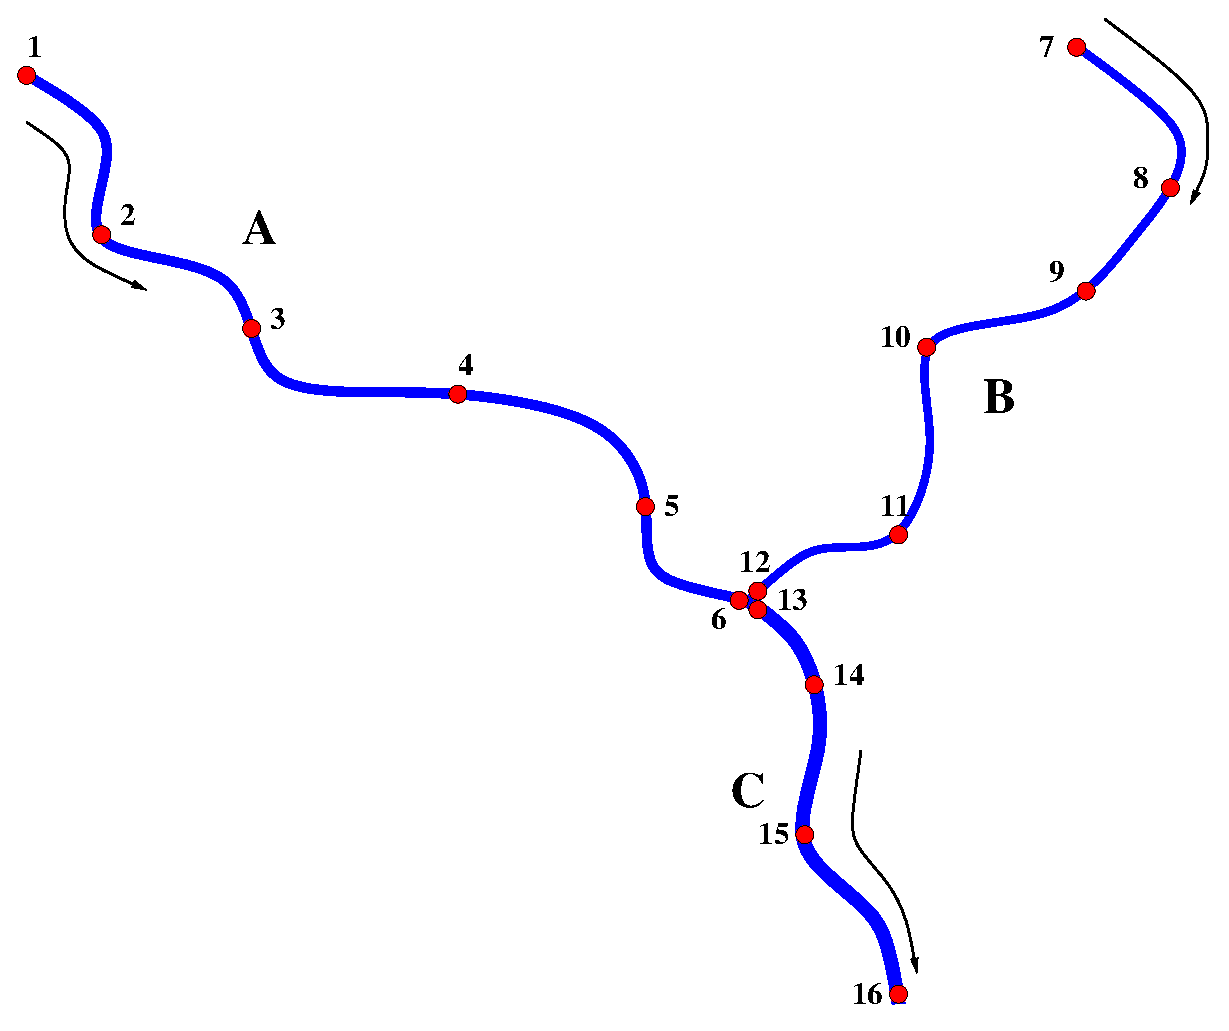
\includegraphics[width=\epswidth, keepaspectratio=true]{Figs/rbd.eps}  }
\caption{An illustrative river network with three branches and the collection of
  computational nodes modeling it}
\label{fig:rivers}
\end{figure}

\subsection{Computational Node}
\label{subsec:node_concept}
In SPRNT, a computational node reflects a position along a river channel where the river
physics behavior is computed. At each node, two variables ($A$ and $Q$) are computed by
solving the related Saint Venant Equations (Eqn.~(\ref{eqn:mass}) and
(\ref{eqn:dynamic})). For example, in Fig.~\ref{fig:rivers}, six nodes are used to model
segment $A$, while 6 nodes are used to model segment $B$.  For each node, besides a unique
node id, the user should also specify at least three other input parameters: {\em slope of
  the reference slope line} ($S_r$), {\em Manning's $n$} and a {\em cross section
  description}. Optionally the user can also provide the elevation of the reference slope
line, the offset of the river bathymetry bottom and the slope reference line if the
reporting of the surface elevation is needed. In addition, users can also provide each
node an X-Y coordinate (usually the GPS coordinate). The coordinates will not be used in
the computation, but merely as references.

\begin{figure}[hbt]
\centerline{
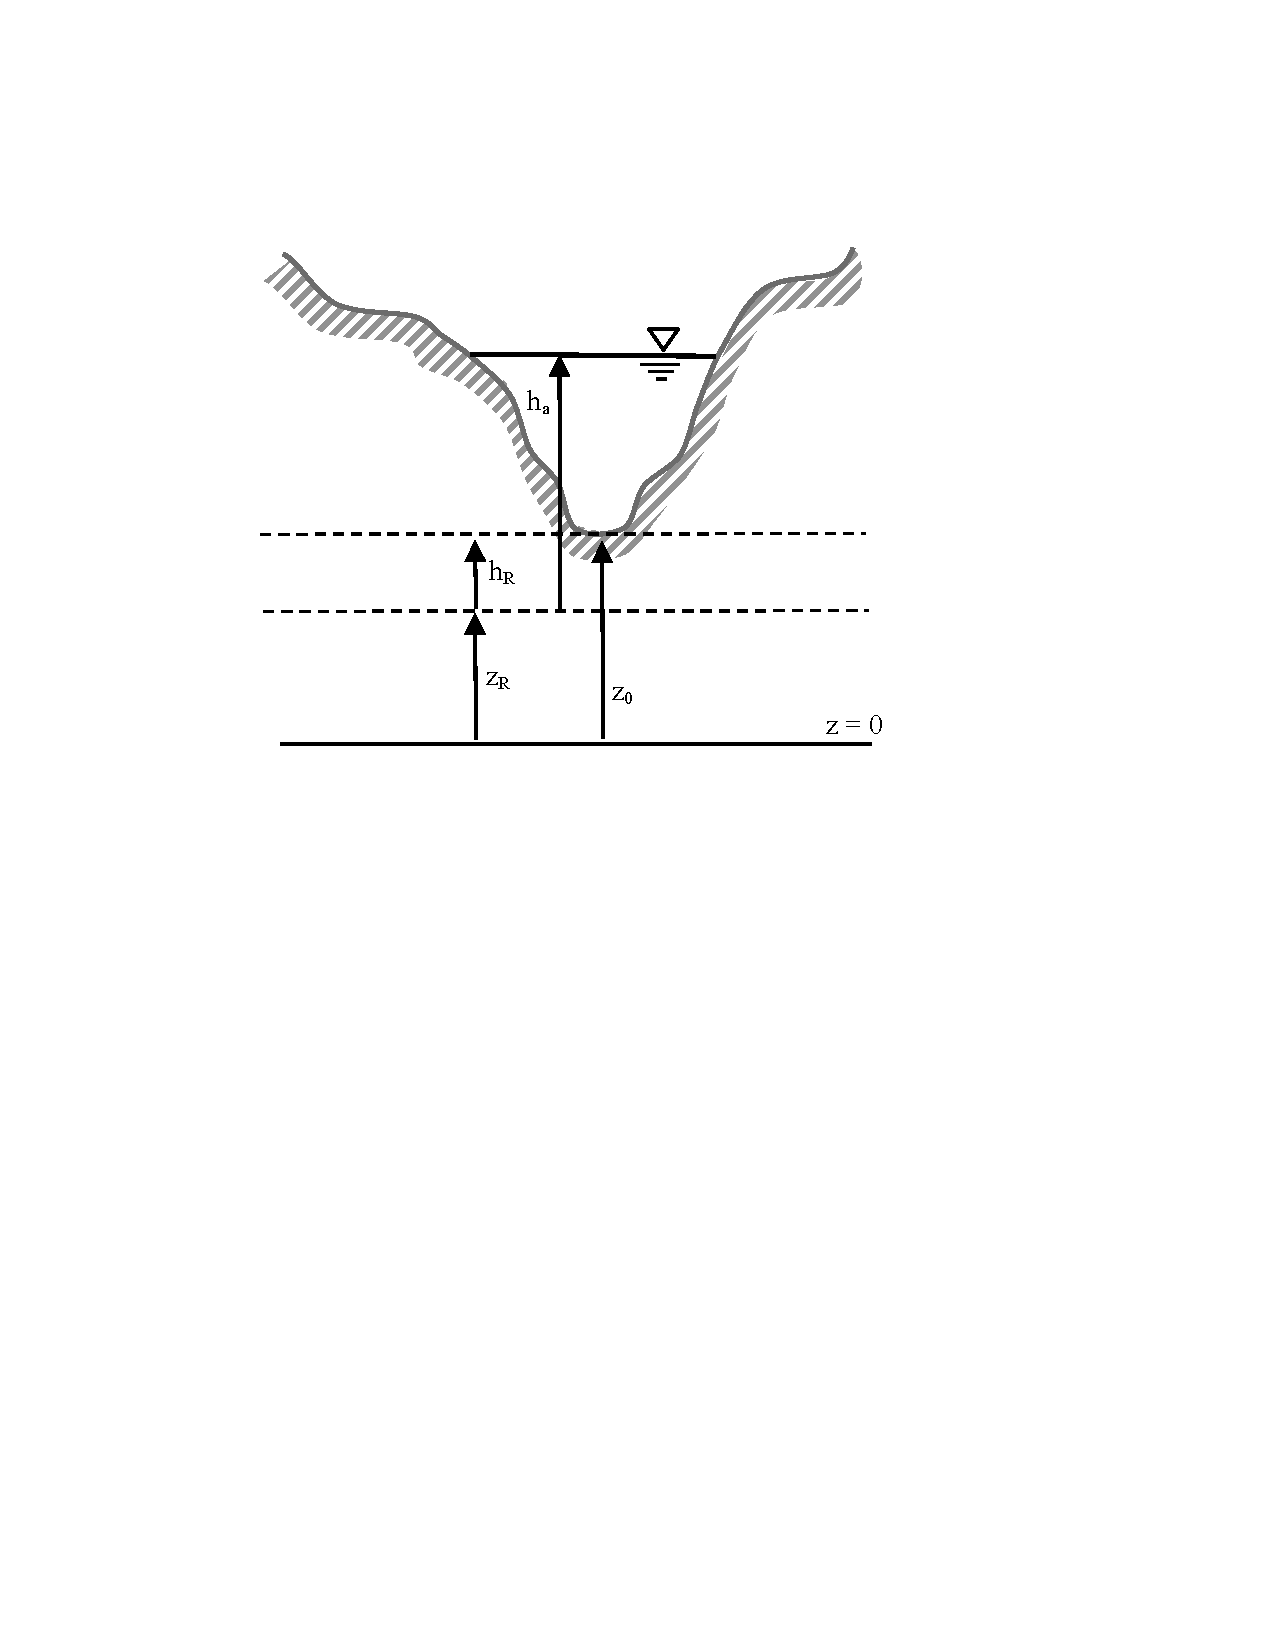
\includegraphics[width=\epswidth, keepaspectratio=true]{Figs/cross_carton.pdf}  
}
\caption{Relationship between bottom elevation, water depth and the surface elevation}
\label{fig:elevation}
\end{figure}

The modeling of the bathymetry data in SPRNT is handled by introducing a ``slope
line''. Refer to the river profile shown in Fig.~\ref{fig:elevation}. We introduce a
smooth ``slope line'' even though the true river bottom profile is jagged. It is expected
that the ``slope line'' has gradually varying slopes which are specified in the netlist as the
$S_R$. At each bathymetry data point, the elevation of the ``slope line'' is the elevation
$Z_R$ (use the datum as the reference). The distance between the true river bottom and
the``slope line'' is the offset $h_R$. Note that in most cases $Z_R$ is positive. However
$h_R$ can be positive or negative. If the ``slope line'' is below the river bathymetry
bottom, then $h_R$ is positive. If the slope line is above the river bathymetry bottom,
then $h_R$ is negative. In either case, the relationship $Z_0 = Z_R + h_R$ always holds.
Fig.~\ref{fig:elevation} provides a visual illustration. Fig.~\ref{fig:sideway} provide a
side view of the river channel, in which at lactation $1$, $h_R$ is positive since the
slope line is below the bathymetry bottom. While at location $2$, $h_R$ is negative since
the slope line is above the bathymetry river bottom.

\begin{figure}[hbt]
\centerline{
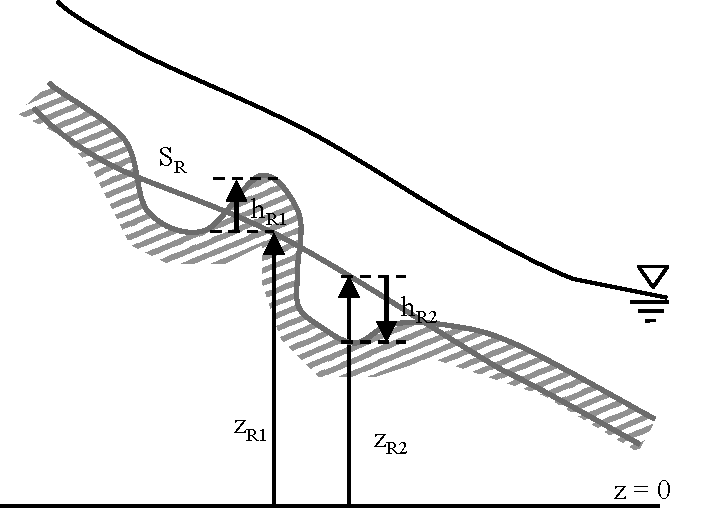
\includegraphics[width=\epswidth, keepaspectratio=true]{Figs/xsec_sideway.pdf}  
}
\caption{Positive $h_R$ and negative $h_R$}
\label{fig:sideway}
\end{figure}


\subsection{Reference Slope}
\label{subsec:bottoms}
The slope of the reference line ($S_R$ line in Fig.~\ref{fig:sideway}) should be consistent with
the river segment length. See Subsection.~\ref{subsec:distance} for further discussions. A
typical value would be between $10^{-2}$ and $10^{-4}$.

\subsection{Manning's $n$}
\label{subsec:manning}
Manning's $n$ is an empirical coefficient to describe the ``resistance'' of the river
segment. A typical value of $n$ would be $0.01$.

\subsection{Cross Section}
\label{subsec:xsec}
Three types of cross sections are supported in SPRNT: rectangular, trapezoidal, and
tabulated xy.

For trapezoidal cross section, it is assumed that two side walls are symmetric. Only two
coefficients are required to specify a trapezoidal cross section: the bottom width
($b_0$) and the side wall slope ($S$, which is defined as the cotangent of the side wall
angle with respect to the horizon). An illustration is shown in Fig.~\ref{fig:trap}. In
this case the slope should be specified as $ctan(\theta)=\frac{0.5}{1.0}=0.5$. For
rectangular cross-section, only the bottom width is needed.
\begin{figure}[hbt]
\centerline{
\includegraphics[width=\epswidth, keepaspectratio=true]{Figs/trap.eps}  
}
\caption{Two coefficients are required to specify a trapezoidal cross section.}
\label{fig:trap}
\end{figure}

A tabulated xy cross section is specified by a table of the Y-Z value across a cut-line
perpendicular to the flow diction. Note that at least three pairs are required to define a
channel. An illustrative example of a tabulated xy cross section is shown in
Fig.~\ref{fig:yz}. In the figure, the red dots are specified in the table. The river bank
cross section is defined by connecting the red dots, as indicated in the black line.
\vspace{0.3in}
\begin{figure}[hb]
\centerline{
\includegraphics[width=\epswidth, keepaspectratio=true]{Figs/yy.eps}}
\caption{An illustrative example of a cross-section described by tabulated XY values.}
\label{fig:yz}
\end{figure}

\subsection{Distance between the Nodes}
\label{subsec:distance}
When the nodes are connected along the river channel, the only set of parameters required
is the distance between two adjacent nodes. Either the meandering distance or the
Euclidean distance can be used. However, the reference slope should be consistent with the
distance.

\subsection{Junction Point}
\label{subsec:junction_pt}
The combination of two upstream tributaries into the downstream branch is described by a
junction point. Physically there is only one point in the natural river for each
junction. In SPRNT, the physical junction point is split into three computational nodes
(nodes 6, 12 and 13 in Fig.~\ref{fig:rivers}). Each node is connected to individual
branches, each of which is described by a set of Saint Venant Equations.  Mass
conservation is applied to the three nodes (For example, water flow rate into node 13
equals the water flowing out of nodes 6 and 12). Another coefficient is required to
describe the flow contributions between the two upstream nodes. For example, if two
branches have equal amount of water flow contribution, then the ratios should be $0.5$ and
$0.5$. However, if branch $A$ contributes $70\%$ of flow into branch $C$, then the ratio
should be $0.7$ and $0.3$. 

\subsection{Forcing Terms}
\label{subsec:forcing}
The forcing terms are the water flows specified at the upstream pour-in points in the river
networks. For the illustrative examples shown in Fig.~\ref{fig:rivers}, forcing terms at
node 1 and 7 are required. Each forcing term is specified as a time series
and should be provided from upstream hydrographs. When there is no water flow inside the
channel, St Venant Equations become singular. Therefore, certain level of small flow is
needed, which is often referred as the ``base flow''. In other words, the forcing terms
should never be smaller than the base flow. Normally a base flow between $0.02 m^3/s$ to
$0.1 m^3/s$ are good choices. 

\subsection{Lateral Inflow}
\label{subsec:lateral}
A lateral inflow can be specified each each node. For example, there
is an inflow between nodes 4 and 5 in Fig.~\ref{fig:flow}. The lateral flow is
applied to the whole segment between two adjacent nodes. For the node at which there is no
lateral inflow defined, it is assumed that the lateral inflow is zero.

\subsection{Downstream Boundary Condition}
\label{subsec:downbd}
A boundary condition specifying the downstream depth is required. In the illustrative
example in Fig.~\ref{fig:flow}, a downstream depth $y$ (or equivalently, the wetted area
$A$) should be specified at node 16. It should be specified as a time series.

\begin{figure}[hbt]
\centerline{
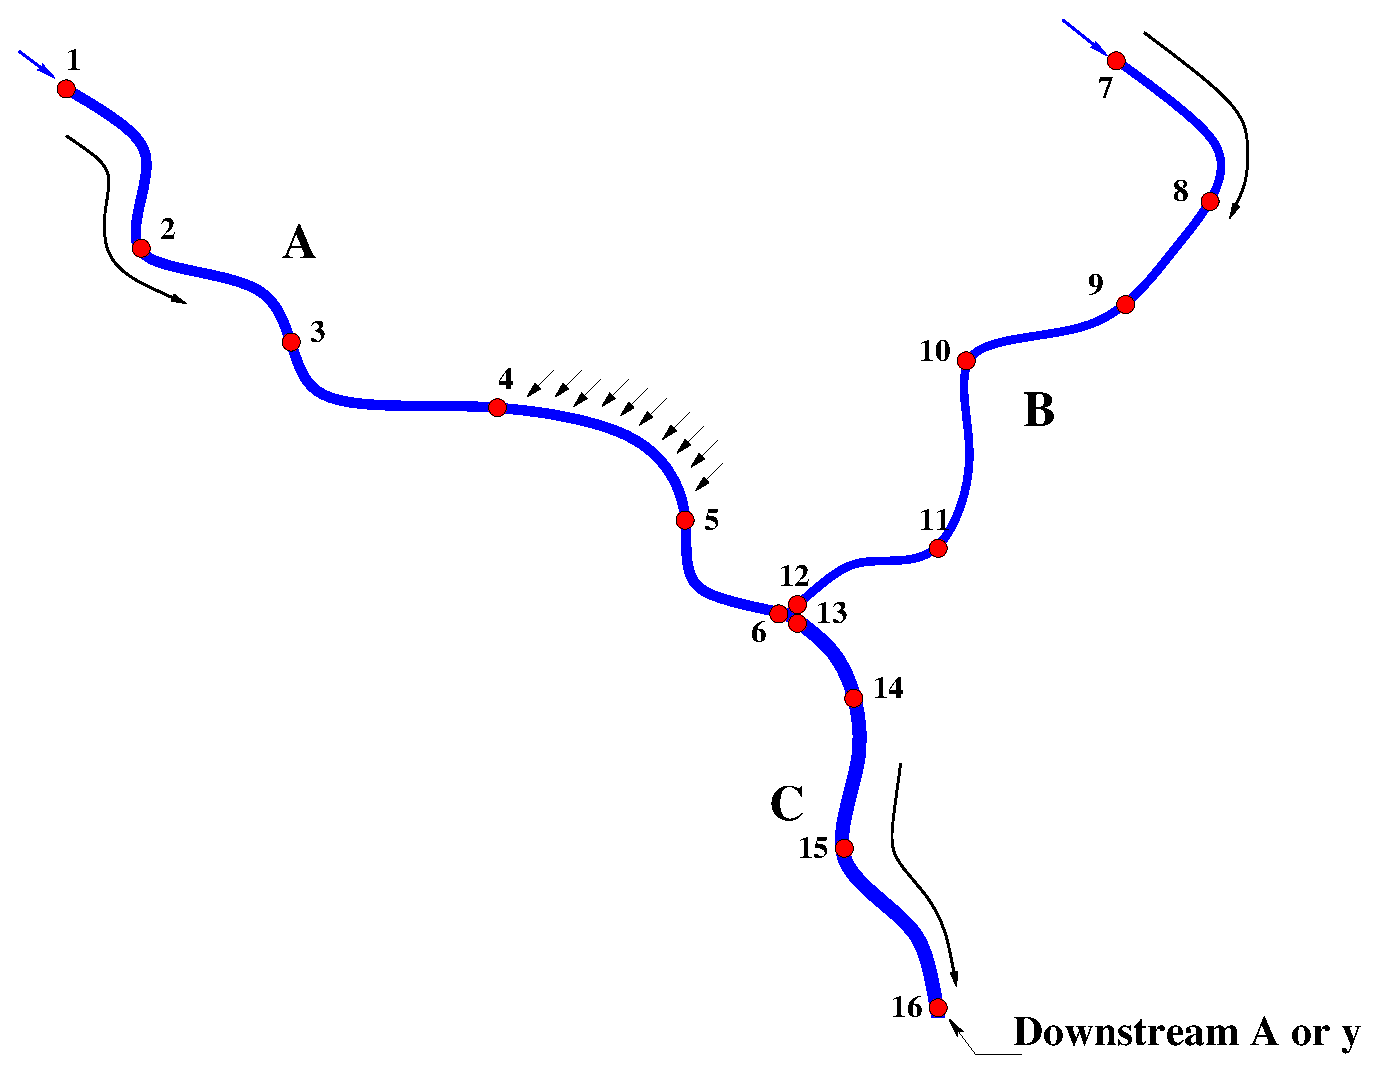
\includegraphics[width=\epswidth, keepaspectratio=true]{Figs/flow.eps}  
}
\caption{The forcing terms, lateral inflow and downstream depth needed to model the flow.}
\label{fig:flow}
\end{figure}



\section{Format of Input Data in Netlist}
\label{sec:netlist}
In SPRNT, the description of the river network is specified in a ``netlist''. Each
netlist consists of the specifications of nodes, segments, branches, forcing terms,
lateral flows, downstream boundary conditions, as well as options which are directives on how the
simulation should be performed. The following is a sample netlist, followed by more detailed
explanations.

\lstset{
  basicstyle=\footnotesize\ttfamily,
  language=C++,
  framexleftmargin=17pt,
  framexrightmargin=10pt,
  numbers=left,numberstyle=\tiny,numbersep=5pt
}
\begin{lstlisting}[firstnumber=1]
## automatically generated by a translation script on Jul 12 2013 15:46:33 CDT
## 
## one segment river bed, test the mixture of xy and trap x-section
## start from base flow 1 and spin down

def options metric=1 end 
def options epoch=2013-12-02T02:30:00Z end
def options TimeStep=60 TimeStepUnit=second end 
def options PrtInterval=2 PrtIntervalUnit=minute end
def options PrtQ=1 PrtA=1 PrtDepth=1 PrtSurfElev=1 PrtCoord = 1 end

def node  id=node_1  sr=0.0083  n=0.04  zr=707.23  hr=0.0 xcoord=123.45 ycoord=567.89
  def xy
    x=0.0 y=6.0
    x=2.5 y=1.0
    x=3.5 y=1.0
    x=6.0 y=6
  end
end

def node  id=2  sr=0.0083  n=0.04  zr=707.23  hr=0.0
  def trapezoidal
    BottomWidth=1 slope=0.5
  end
end

def node  id=3  sr=0.0083  n=0.04  zr=707.23  hr=0.0
  def xy
    x=0.0 y=6.0
    x=2.5 y=1.0
    x=3.5 y=1.0
    x=6.0 y=6
  end
end

def node  id=4  sr=0.0083  n=0.04  zr=707.23  hr=0.0
  def trapezoidal
    BottomWidth=1 slope=0.5
  end
end

def node  id=5  sr=0.0083  n=0.04  zr=707.23  hr=0.0
  def xy
    x=0.0 y=6.0
    x=2.5 y=1.0
    x=3.5 y=1.0
    x=6.0 y=6
  end
end

def node  id=6  sr=0.0083  n=0.04  zr=707.23  hr=0.0
  def xy
    x=0.0 y=6.0
    x=2.5 y=1.0
    x=3.5 y=1.0
    x=6.0 y=6
  end
end


def segment up=node_1 down=2 Length=40 end
def segment up=2 down=3 Length=40 end
def segment up=3 down=4 length=40 end
def segment up=4 down=5 length=40 end
def segment up=5 down=6 length=40 end

def qsource
  location=node_1 
  def TimeSeries
    TimeUnit=minute
    t=0 v=1.0
    t=1 v=1.0
    t=2 v=0.5
    t=4 v=0.1
    t=6 v=0.5
    t=80 v=0.1
    t=100 v=0.1
    t=1000 v=0.1
    t=1200 v=0.5
    t=1400 v=1.0
    t=2500 v=1.0
    t=5000 v=1.0
  end
end


def BoundaryCondition
  location=6 type=area
  def timeseries
    TimeUnit=minute
    t=0 v=1
    t=2800 v=1
  end
end

def options
  StopTime=8 StopTimeUnit=minute
end

## end
\end{lstlisting}

\subsection{General Syntax}
\label{subsec:syntax}
A SPRNT netlist consists of many blocks, each block is defined by two keywords: {\tt def}
and {\tt end}. Within each {\tt def} and {\tt end} block, the values are specified by {\tt
keyword = value} pairs. Multiple {\tt keyword = value} pairs are allowed, depending on the
requirement of the specific block. Also {\tt def} and {\tt end} block can be nested, again depends
on the nature of the block.  Note that the two keywords are \underline{case
  insensitive}. Therefore, it is perfectly legal to use {\tt Def}--{\tt End} or {\tt
  DEF}--{\tt END} to define the blocks. Or {\tt dEf}--{\tt EnD}.


\subsection{Top-Level Functional Blocks}
\label{subsec:toplevel}
The functional keyword immediately following the {\tt def} keyword defines the nature of the
top-level block. In the current version there are seven top-level keywords to
define the blocks {\tt node},{\tt segment},{\tt junction},{\tt qsource}, {\tt
  lateralsource}, {\tt boundarycondition} and {\tt options}. Note that the functional
keywords are also \underline{case insensitive}. For better readability, it is perfectly
fine to use {\tt BoundaryCondition} instead of {\tt boundarycondition}. 

\subsection{Secondary Level Functional Blocks}
\label{subsec:secondlevel}
Within each top-level block, it may be necessary to include secondary functional blocks by
nesting {\tt def}--{\tt end} blocks. The following secondary functional blocks are needed
when specifying nodes: {\tt trapezoidal}, {\tt rectangular}, {\tt xy}. A {\tt timeseries}
subblock is needed when defining {\tt qsource},{\tt lateralsource} and {\tt
  boundarycondition}. Again the secondary functional keywords are also \underline{case
  insensitive}.

\subsection{Single Line Format}
\label{subsec:single}
It is preferred to have the keywords {\tt def} and {\tt end} the first word in a new
line. However, it is allowed to have empty space ahead of the keywords to enhance
readability, which could be useful for nested blocks. In the case of short blocks, it is
allowed to have one-line {\tt def}--{\tt end} blocks, such as in the {\tt options} and {\tt
  segment} blocks. Examples can be found in the example above.

\subsection{Keyword--Value Pairs}
\label{subsec:kvpair}
Within each block, the values are specified as {\tt keyword = value} pairs. Usually more
than one pairs are needed to completely define the specification. The sequence of those pairs
has no effect. For example, the pair {\tt def options metric=1 prtq=1 end} has the exactly
same effect as {\tt def options prtq=1 metric=1 end}. Both of them indicate that the
flow rate Q will be printed, and the netlist is specified using metric units. More details
are provided later in this section.

\subsection{Comments and Empty Lines}
\label{subsec:comments}
Empty lines will be ignored. Any lines starting with an number sign (\#) will be treated
as comments and ignored. The asterisk (*) and percentage sign (\%) can also be used to
indicate comments. Be careful that the comment sign should be the very first character in
the comment line. To make the netlist readable, it is always a good habit to leave some
comments in the netlist for future reference.

\subsection{Node}
\label{subsec:node}
To define a node, the block should be defined as {\tt def node}, {\tt end}. Each block
defines a unique node on the river channel. The following keywords are available within a {\tt
node} block:

\subsubsection{Id}
\label{subsubsec:id}
Required. Defines the id of the node. As with other keywords, it is \underline{case
  insensitive}. Therefore the exact keyword could be {\tt id}, {\tt Id} or other
combination. It should be followed by the name of the node as {\tt id=node\_name}. The
node name should:
\begin{itemize}
\item{Be numeric or alphabetic}
\item{Be less than 60 characters long}
\item{NOT contain equal sign (=), colon(:), semi-colon(;), comma (,), space, or tab}.
\end{itemize}
A convenient approach is to use underscore (\_) to replace space. Also note that that
unlike the keyword (``id''), the node names are 
\underline{case sensitive}. Therefore a node with the name of \\
{\tt crossing\_@\_first\_\&\_51st\_street}\\
will be considered a different node compared to \\
{\tt crossing\_@\_first\_\&\_51ST\_Street}.

\subsubsection{SR}
\label{subsubsec:s0}
Required. Specifies the slope of the ``slope line'' at the node. It should be followed by
a real number. Scientific notation is allowed. Hence it can be {\tt s0=0.00012} or {\tt s0
  = 1.2e-4}.

\subsubsection{N}
\label{subsubsec:n}
Required. This is the Manning's n at the node. It should be followed by a real number.

\subsubsection{ZR}
\label{subsubsec:z0}
Required. This is the elevation of the ``slope line'' relative to the datum for the $s_R$
line. It should be followed by a real number. Normally a positive number is used since the
datum is always the lowest point. But in reality any real values can be used.

\subsubsection{HR}
\label{subsubsec:h0}
Required. This is the relative elevation of the $s_R$ line with respect to the true river
bed bottom. It should be followed by a real number. Depends on the relative position of
the river bottom, it could be either positive or negative.

\subsubsection{Xcoord}
\label{subsubsec:xcoord}
Optional. This is the x-coordinate of the node when looked from above. It should be
followed by a real number. The value of the x-coordinate is not used in the
simulation. It is only useful when printing the solutions. The default value is -1.

\subsubsection{Ycoord}
\label{subsubsec:ycoord}
Optional. Y-coordinate of the node. Same as the x-coordinate.

\subsection{Cross section block}
\label{subsubsec:xsec}
Each node should have at least one of the three cross section specifications: {\tt
  rectangular}, {\tt trapezoidal} or {\tt xy}. Note that two {\tt end} keywords are needed
at end of the specification.

\subsubsection{Rectangular}
\label{subsubsec:rect}
Specifies a rectangular cross section. Currently the only keyword is {\tt
  bottomwidth}. Again the keyword is case insensitive. Therefore it is more readable to
use {\tt BottomWidth}. It should be followed by a positive real number. 

\subsubsection{Trapezoidal}
\label{subsubsec:trap}
Specifies a trapezoidal cross section. Two keywords are required {\tt bottomwidth} and
{\tt slope}. The slope is the ratio between the offsets and is dimensionless.

\subsubsection{XY}
\label{subsubsec:xy}
Specifies a XY cross section. It is specified by a table of the relative distance on the
cut-line on the river (X) with the relative elevation of each point (Y). The length of
each {\tt XY} block can be arbitrary, but should have at least 3 entries. (Two points
only define a straight line and does not define a channel).

\subsection{Segment}
\label{subsec:segment}
The {\tt segment} block defines a segment, which connects two adjacent nodes along the channel. The 
keywords are:

\subsubsection{Up}
\label{subsubsec:up}
Required. Specifies the upstream node. If the upstream node is not defined by a
{\tt node} block, an error will occur. The matching is performed by comparing the node
names.

\subsubsection{Down}
\label{subsubsec:down}
Required. Specifies the downstream node. 

\subsubsection{Length}
\label{subsubsec:length}
Required. Specify the length of the segment. The unit is determined by the Metric option.

\subsection{Junction}
\label{subsec:junction}
Specifies how two branches should be merged. The current implementation uses a linear
mixing scheme. The keywords are:

\subsubsection{Up1}
\label{subsubsec:up1}
Required. The name of the first upstream node.

\subsubsection{Up2}
\label{subsubsec:up2}
Required. The name of the second upstream node.

\subsubsection{Down}
\label{subsubsec:downn}
Required. The name of the downstream node.

\subsubsection{Coeff1}
\label{subsubsec:coeff1}
Required. The mixing coefficient associated with the first upstream node. The required
value should be a positive real number.

\subsubsection{Coeff2}
\label{subsubsec:coeff2}
Required. The mixing coefficient associated with the second upstream node. 
\\
Here is an example of the {\tt junction}:\\
{\tt def junction down=n100 up1=n80 up2=n20 coeff1=0.45 coeff2=0.55 end}\\
The above statement means that the reach ended with node {\tt n80} merges with the reach
ended with node {\tt n20} and pours into the reach started with node {\tt n100}. The mixing
coefficients are $0.45$ and $0.55$ respectively.


\subsection{Qsource}
\label{subsec:qsources}
A {\tt qsource} block defines a Q source at the upstream pour-in points of the
network. It is defined by a location as well as a time-series.

\subsubsection{Location}
\label{subsubsec:location1}
Required. It should be followed by the node name where it is applied. This particular node
should be the first node in the reach.

\subsubsection{TimeSeries}
\label{subsubsec:ts} 
Required. The length of the block can be arbitrary, but it
should be at least of length of two. Two keywords are required, time {\tt t}
and value {\tt v}. It also requires a field to specify the unit of
the time by using the keyword {\tt TimeUnit}. The possible options are {\tt second},
{\tt minute} or {\tt hour}. The unit of the values (flow rate Q) is determined by the
Metric in option.

\subsection{LateralSource}
\label{subsec:lsources}
A {\tt LateralSource} block defines a lateral Q source. It has exactly same syntax as the
Qsource. The difference is that the lateral inflow will be applied to the segment
connecting two adjacent nodes.

\subsection{BoundaryCondition}
\label{subsec:bcondition}
A {\tt BoundaryCondition} block defines the boundary condition at the downstream
node. It requires three keywords:

\subsubsection{Location}
\label{subsubsec:location2}
Required. Should a node name.

\subsubsection{Type}
\label{subsubsec:type}
Required. SPRNT supports two type of boundary conditions, either wetted area (use {\tt
area}) , or the equivalent depth (use {\tt depth}).

\subsubsection{TimeSeries}
\label{subsubsec:ts2} 
Required. It defines a time-series to specify time-varying boundary condition. A constant boundary
condition can be specified by a time series with only two entries, with identical {\tt v} values. The
unit of provided value is determined by the Metric option.


\subsection{Options}
\label{subsec:options}
The option block is applied to control the behavior of the simulation. An option block is
defined by keyword {\tt options}. Note that multiple {\tt options} blocks can be
specified. The net effects are additive. If conflicting options are specified, the last
one will be effective.

\subsubsection{Stoptime}
\label{subsubsec:stoptime}
Required. This is the only required field among the options. It specifies for how long the
dynamic simulation should be performed. It should be specified by a real number.

\subsubsection{StoptimeUnit}
\label{subsubsec:stoptimeu}
Optional. The unit of the stop time specified above. The possible options are {\tt second},
{\tt minute} and {\tt hour}. The default value is second.

\subsubsection{Timestep}
\label{subsubsec:timestep}
Optional. Default value is 0. The time step used in unsteady simulation. If zero is
specified, SPRNT will automatically determine the optimal time step to be used. If a
nonzero value is specified, SPRNT will honor the specified time step by not taking any
time steps larger. However, SPRNT may take smaller time steps when the river physics
behavior requires so. In other words, the provide time step is just the upper bound of
real time steps.  \underline{Caution}: excessively small time step could make the
simulation very slow. For example, simulating a 7-day event at time step of 1 second will
require 604,800 time points, which could take a long time to finish.

\subsubsection{TimestepUnit}
\label{subsubsec:timestepunit}
Optional. The unit of the time step specified. Default value is second.

\subsubsection{PrtInterval}
\label{subsubsec:prtint}
Optional. Specifies how often the solutions should be printed. Note that the printing
interval is different from the simulation time step.  The printing interval at a fixed
value.  \underline{Caution}: excessively small print interval can generate very large disk
files and can slow down the overall simulation time. When zero value is
specified, the results will be printed based on raw simulation time steps. Default value is
zero.

\subsubsection{PrtIntervalUnit}
\label{subsubsec:prtintunit}
Optional. Default value is second. The unit used to specify the print interval above.

\subsubsection{PrtStart}
\label{subsubsec:prtstart}
Optional. Default value is 0. The value specifies the starting time when the dynamic
simulation is required to store. The dynamic simulation always start at time point
0. However, in certain circumstances it is desirable to ignore some of the earlier
results. This value is used to specify the starting time for print.

\subsubsection{PrtStartUnit}
\label{subsubsec:prtsttunit}
Optional. Default value is second. The unit of the above specification.

\subsubsection{PrtQ}
\label{subsubsec:prtq}
Optional. Default value is 0. The value should be specified either 0 or 1. When the flag
is specified, the flow rate Q at each node will be printed in the result file. Note that
the printing behavior is further controlled by {\tt PrtInterval} and {\tt PrtStart}. 

\subsubsection{PrtA}
\label{subsubsec:prta}
Optional. Default value is 0. The value should be specified either 0 or 1. When the flag
is specified, the wetted area at each node will be printed in the result file.

\subsubsection{PrtDepth}
\label{subsubsec:prtd}
Optional. Default value is 0. The value should be specified either 0 or 1. When the flag
is specified, the depth at each node will be printed in the result file.

\subsubsection{PrtSurfElev}
\label{subsubsec:prtsfe}
Optional. Default value is 0. The value should be specified either 0 or 1. When the flag
is specified, the surface elevation at each node will be printed in the result file. Note
that at least one of the above four flags have to be selected in order to enable the Ge nation of
the result file.

\subsubsection{PrtCoord}
\label{subsubsec:prtcoord}
Optional. Default value is 0. The value should be specified either 0 or 1. When the flag
is specified, the x- and y-coordinate of each node will be printed along with the other
specified quantities.


\subsubsection{CheckOnly}
\label{subsubsec:co}
Optional. Default value is 0. The value should be specified either as 0 or 1. When the
flag is turned on, SPRNT will only perform a topological check and will not perform the
simulation at all.  This could be useful for quick debug of the netlist.

\subsubsection{SSFile}
\label{subsubsec:ssf}
Optional. Default value is empty. It should be followed by a file-name. If such a file-name
is specified, SPRNT will try to locate file which contains the steady-state solutions of
the given river network. If it is found, the content of the file will be loaded into
SPRNT as the suggestions for steady-state solutions. If the file is specified,
the computed steady-state solutions will be stored in the file for later use.
The content of the SSFile should not be tempered with in any way.

\subsubsection{Metric}
\label{subsubsec:metric}
Optional. Default value is 0. The value should be either 0 or 1. When the flag is
specified as 1 , the netlist is in metric units. In particular, the flow rate will be in
$m^3/s$, the length and depth will be in $m$, and the wetted area will be in $m^2$. When
the flag is not specified (0), the flow rate will be in $f^3/s$, the length and depth will
be in $ft$ and the wetted area will be in $ft^2$.  This option will also affect how the
results are stored.

\subsubsection{Verbose}
\label{subsubsec:verbose}
Optional. Default value is 0. If the value is set to 1, more status reports will be
printed on the screen during the steady and unsteady solution steps.

\subsubsection{Epoch}
\label{subsubsec:epoch}
Optional. Default value is 1970-01-01T00:00:00Z. SPRNT always starts simulation from time
point 0. The epoch time indicates the real-world time this time point 0 refers to. The
value will not be used within SPRNT. Instead it will be simply printed in the output file
for reference. The value is treated as a string, therefore the format is
arbitrary. However, it should not contain any space (' '), equal sign (=), comma (,), or
period (.). The default value is the epoch time on Unix systems, which corresponds to 00
hour UTC on January 1st, 1970. 

\section{SPRNT Output of the Sample Netlist}
\label{sec:output}
The output of the previous netlist is as follows:
\begin{lstlisting}[firstnumber=1]
*** SPRNt Results. Netlist: "test.spt" Epoch: "2013-12-02T02:30:00Z" Reqested Tstop: 8 min
*** id time(min) flow(m3/s) wet_a(m2) depth(m) surf_elev(m) xy-coordinates
node_1 0 1.000000e+00 8.767511e-01 6.593638e-01 7.078893e+02 123.4500 567.8900
2 0 1.000000e+00 8.767403e-01 6.593615e-01 7.078893e+02 -1.0000 -1.0000
3 0 1.000000e+00 8.767709e-01 6.593758e-01 7.078894e+02 -1.0000 -1.0000
4 0 1.000000e+00 8.764441e-01 6.591830e-01 7.078892e+02 -1.0000 -1.0000
5 0 1.000000e+00 8.815245e-01 6.622367e-01 7.078922e+02 -1.0000 -1.0000
6 0 1.000000e+00 1.000000e+00 7.320598e-01 7.079620e+02 -1.0000 -1.0000
*** id time(min) flow(m3/s) wet_a(m2) depth(m) surf_elev(m) xy-coordinates
node_1 2 5.000000e-01 5.799957e-01 4.696818e-01 7.076997e+02 123.4500 567.8900
2 2 6.633108e-01 6.835633e-01 5.385469e-01 7.077685e+02 -1.0000 -1.0000
3 2 7.707245e-01 7.477068e-01 5.796802e-01 7.078097e+02 -1.0000 -1.0000
4 2 8.428390e-01 7.891648e-01 6.057178e-01 7.078357e+02 -1.0000 -1.0000
5 2 8.920259e-01 8.212431e-01 6.255824e-01 7.078556e+02 -1.0000 -1.0000
6 2 9.121197e-01 1.000000e+00 7.320598e-01 7.079620e+02 -1.0000 -1.0000
*** id time(min) flow(m3/s) wet_a(m2) depth(m) surf_elev(m) xy-coordinates
node_1 4 1.000000e-01 2.016738e-01 1.846242e-01 7.074146e+02 123.4500 567.8900
2 4 2.246723e-01 3.282551e-01 2.870549e-01 7.075170e+02 -1.0000 -1.0000
3 4 3.348487e-01 4.297309e-01 3.636133e-01 7.075936e+02 -1.0000 -1.0000
4 4 4.381515e-01 4.984963e-01 4.131499e-01 7.076431e+02 -1.0000 -1.0000
5 4 5.218083e-01 6.238072e-01 4.992042e-01 7.077292e+02 -1.0000 -1.0000
6 4 5.545738e-01 1.000000e+00 7.320598e-01 7.079620e+02 -1.0000 -1.0000
*** id time(min) flow(m3/s) wet_a(m2) depth(m) surf_elev(m) xy-coordinates
node_1 6 5.000000e-01 5.033456e-01 4.165868e-01 7.076466e+02 123.4500 567.8900
2 6 4.114452e-01 4.408587e-01 3.717570e-01 7.076017e+02 -1.0000 -1.0000
3 6 3.558093e-01 4.161239e-01 3.536064e-01 7.075836e+02 -1.0000 -1.0000
4 6 3.407731e-01 3.876073e-01 3.323718e-01 7.075624e+02 -1.0000 -1.0000
5 6 3.462465e-01 5.531844e-01 4.513355e-01 7.076813e+02 -1.0000 -1.0000
6 6 3.494974e-01 1.000000e+00 7.320598e-01 7.079620e+02 -1.0000 -1.0000
*** id time(min) flow(m3/s) wet_a(m2) depth(m) surf_elev(m) xy-coordinates
node_1 8 4.891892e-01 5.184549e-01 4.272165e-01 7.076572e+02 123.4500 567.8900
2 8 4.836288e-01 5.101433e-01 4.213679e-01 7.076513e+02 -1.0000 -1.0000
3 8 4.688917e-01 5.020420e-01 4.156659e-01 7.076456e+02 -1.0000 -1.0000
4 8 4.469708e-01 4.679022e-01 3.913319e-01 7.076213e+02 -1.0000 -1.0000
5 8 4.276960e-01 5.926982e-01 4.782997e-01 7.077083e+02 -1.0000 -1.0000
6 8 4.208896e-01 1.000000e+00 7.320598e-01 7.079620e+02 -1.0000 -1.0000
\end{lstlisting}

The comments in lines 1, 8, 15, 22 and 29 explain the meaning of each field and their
units. Note only the first node ``node\_1'' has x- and y-coordinates. The x- and
y-coordinates are not specified. Therefore the default value of -1 is printed.

\end{document}

%% that's all, folks
%% 
%% Local Variables:
%% mode: LaTex
%% End:
%% 
